In our basic extrapolation framework, we trained networks on predicting the exact ground-state energy given a few sequences of absoulte energy values. This method is inherently dependent on the absolute values of the energy, since the networks fundamentally consist of linear maps from one layer to the next. Nuclear ground-state energies have a very broad range, which we already saw in our inspected nuclei. For example, \n{2}{H} has a ground-state energy of approximately \SI{-2.1}{\mega\electronvolt} and \n{4}{He} has a ground-state energy of approximately \SI{-28.4}{\mega\electronvolt}, based off the NCSM calculations shown in \autoref{fig:example_nmax} and \autoref{fig:eval_extended}. As a result, we cannot confidentially exclude the possibility of the absolute ground-state energies influencing the network predictions.

In this chapter, we want to analyze the influence of the absolute energies on the network prediction by implementing a different extrapolation method based on our previous framework, which will work by extrapolating the differences of the energy sequences.
\section{framework}
In order to implement our difference based extrapolation framework, we have to think about how we have to change the generation of the input data, the network structure as well as the extrapolation process of our basic extrapolation framework.

We want to base our network training on the same data set as the basic framework. The networks now should get the differences of consecutive ground-state energies in the sequences as an input. To achieve this, we generate the same formatted input sequences out of the raw NCSM calculations, using the inflation algorithm described in \autoref{sec:inflate}. The formatted input data thus consists of four consecutive energy values for three oscillator frequencies, as well as a limit which will be used to compute the prediction target of our networks. To turn those sequences into our input difference sequences, we calculate the three differences between the four energy values. When the networks get input data in the form of energy differences, they cannot possibly predict an absolute ground-state energy from them. This means that the prediction target will also have to be modified to a difference. It is natural to take the difference between the last value of the energy sequence and the limit as a target. However, this leads to a problem, as the limit is the same for the three oscillator frequencies for a given nucleus and interaction, but the last values of the energy sequences can vary depending on the frequency. Because the three difference sequences are all put into a network simultaneously, we have to find a single common extrapolation target. For this, we decide to take the difference between the mean of the last values for all three sequences and the limit.

Note that, since we now only have three direct inputs available, which consist of the differences of the four absolute values, the network structure has to be adjusted to be compatible with this data. For the input layer, we have $L^{(1)} = 3 \times 3 = 9$ input neurons. Furthermore, we reduce some of the hidden neurons in the hidden layers to accommodate the reduced input neurons. We empirically decide on $L^{(2)} = 18$, $L^{(3)} = 12$. The single output neuron stays the same. We could have chosen to keep the network structure the same, but this would require to input four differences of five energies, which would mean that those networks got more information about the sequences. To ensure comparability, we chose to keep the information the same but adjust the network structure.

Further modifications include the adjustment of our sequence shifting. In our basic framework, we decided to shift the formatted sequences by a random amount of $[\SI{-10}{\mega\electronvolt}, \SI{10}{\mega\electronvolt}]$ to counter the dependency on absolute values. They are no longer needed, as they would cancel out when calculating the differences. Also, the threshold for deeming a network valid is reduced to \SI{0.1}{\mega\electronvolt}, as the energy differences which are input are generally much smaller than the absolute values.

To compensate for the shift in the training set, we also have to modify the evaluation of a network. The evaluation will work the same way as in our basic framework, but now, the final prediction is calculated by adding the mean of the last energy values back onto the network prediction.

\section{results and comparison}
Using our newly constructed difference-based extrapolation framework, we can now do the same analysis on our three nuclei \n{2}{H}, \n{3}{H} and \n{4}{He} using the same interaction as used earlier. Even though the difference-based framework computes a difference prediction internally, the final evaluation will still base off the same absolute energy differences and result in an absolute energy prediction. This means that we can apply our different evaluation modifications from \autoref{chap:extended} and discuss the influences of them on the difference based evaluation. Furthermore, using the same nuclei allows us to compare the difference based extrapolation and the absolute value extrapolation.

The results of our difference based extrapolation is shown in \autoref{fig:eval_diff}. The final extrapolated values and their uncertainty are shown in \autoref{tab:eval_diff} as well for each $N_\mathrm{max}$ and each SRG flow parameter.

% Generell: Predictions VIEL genauer, besonders bei hohem Nmax
Looking at all three nuclei, we can see that the uncertainty of all training modes is drastically reduced. Especially for higher $N_\mathrm{max}$, the predictions get very precise. Furthermore, the absolute value of the predictions are generally way closer to a reasonable limit. This can be seen for the nuclei \n{4}{He} and \n{3}{H}, where the networks trained with the unmodified or the $N_\mathrm{max}$-limitation training mode in the absolute based extrapolation framework predicted unreasonably low values for all $N_\mathrm{max}$. This could be caused by the fact that the absolute values are purged from the resulting differences, such that the absolute value of the sequences do not matter in the extrapolation process. This leads to a focus on the convergence of the sequences. When the sequence converges, the differences tend towards zero, such that evaluation yields a prediction for the ground-state energy close to the last values in the inputted sequences. There is a disadvantage of the difference-based extrapolation in the nucleus \n{4}{He} for a flow parameter of $\alpha = \srg{0.04}$. Here, the sequences converge fast, but for the small values of $N_\mathrm{max}$ given, the sequences are cut off for the lower oscillator frequencies of $\hbar\Omega = \SI{12}{\mega\electronvolt}$ and \SI{14}{\mega\electronvolt}. This leads to the network recieving a broad range of differences, resulting in a greater uncertainty for the ground-state energy prediction. We can also see that this effect gets better for $\alpha = \srg{0.08}$, where even the sequences for the lower oscillator frequencies are now visibly more converged to the limit.

% H2: 0.08 schlechter als 0.04

\begin{table}[H]
  \caption{Extrapolation results in \si[]{\mega\electronvolt} of the difference based framework for the nuclei \n{2}{H} \textbf{(a)}, \n{3}{H} \textbf{(b)} and \n{4}{He} \textbf{(c)}. For each interaction characterized by the flow parameter $\eta = \srg{0.04}, \srg{0.08}$, the final extrapolation results for the given $N_\mathrm{max}$ value is shown. Here, \textbf{(1)} is our basic extrapolation without further modifications of the training step, \textbf{(2)} is the $N_\mathrm{max}$-limitation training mode, \textbf{(3)} is the SRG-filter training mode. }
  \label{tab:eval_diff}
  \centering
  \begin{subtable}{\textwidth}
    \caption{}
    \centering
    \begin{tabular}{
        r|
        S[table-format=-2.3(3)]
        S[table-format=-2.3(3)]
        S[table-format=-2.3(3)]
        S[table-format=-2.3(3)]
        S[table-format=-2.3(3)]
        S[table-format=-2.3(3)]
      }
      \toprule
      $\eta$                           &
      \multicolumn{3}{c}{$\srg{0.04}$} &
      \multicolumn{3}{c}{$\srg{0.08}$}   \\
      \midrule
      $N_\mathrm{max}$                 &
      {8}                              &
      {10}                             &
      {12}                             &
      {8}                              &
      {10}                             &
      {12}                               \\
      \midrule
      (1)                              &
      -2.066 \pm 0.065                 &
      -2.144 \pm 0.025                 &
      -2.129 \pm 0.022                 &
      -2.054 \pm 0.069                 &
      -2.113 \pm 0.028                 &
      -2.126 \pm 0.023                   \\
      (2)                              &
      -2.080 \pm 0.055                 &
      -2.146 \pm 0.023                 &
      -2.127 \pm 0.020                 &
      -2.064 \pm 0.056                 &
      -2.110 \pm 0.026                 &
      -2.124 \pm 0.022                   \\
      (3)                              &
      -2.068 \pm 0.055                 &
      -2.153 \pm 0.038                 &
      -2.149 \pm 0.034                 &
      -2.062 \pm 0.041                 &
      -2.124 \pm 0.032                 &
      -2.158 \pm 0.036                   \\
      \bottomrule
    \end{tabular}
  \end{subtable}
  \par\bigskip
  \begin{subtable}{\textwidth}
    \caption{}
    \centering
    \begin{tabular}{
        r|
        S[table-format=-2.3(3)]
        S[table-format=-2.3(3)]
        S[table-format=-2.3(3)]
        S[table-format=-2.3(3)]
        S[table-format=-2.3(3)]
        S[table-format=-2.3(3)]
      }
      \toprule
      $\eta$                           &
      \multicolumn{3}{c}{$\srg{0.04}$} &
      \multicolumn{3}{c}{$\srg{0.08}$}   \\
      \midrule
      $N_\mathrm{max}$                 &
      {8}                              &
      {10}                             &
      {12}                             &
      {8}                              &
      {10}                             &
      {12}                               \\
      \midrule
      (1)                              &
      -8.453 \pm 0.099                 &
      -8.528 \pm 0.044                 &
      -8.470 \pm 0.026                 &
      -8.410 \pm 0.090                 &
      -8.465 \pm 0.035                 &
      -8.460 \pm 0.025                   \\
      (2)                              &
      -8.461 \pm 0.082                 &
      -8.526 \pm 0.036                 &
      -8.468 \pm 0.025                 &
      -8.422 \pm 0.074                 &
      -8.464 \pm 0.031                 &
      -8.457 \pm 0.023                   \\
      (3)                              &
      -8.390 \pm 0.064                 &
      -8.493 \pm 0.028                 &
      -8.466 \pm 0.026                 &
      -8.408 \pm 0.045                 &
      -8.460 \pm 0.026                 &
      -8.466 \pm 0.025                   \\
      \bottomrule
    \end{tabular}
  \end{subtable}
  \par\bigskip
  \begin{subtable}{\textwidth}
    \caption{}
    \centering
    \begin{tabular}{
        r|
        S[table-format=-2.3(3)]
        S[table-format=-2.3(3)]
        S[table-format=-2.3(3)]
        S[table-format=-2.3(3)]
        S[table-format=-2.3(3)]
        S[table-format=-2.3(3)]
      }
      \toprule
      $\eta$                           &
      \multicolumn{3}{c}{$\srg{0.04}$} &
      \multicolumn{3}{c}{$\srg{0.08}$}   \\
      \midrule
      $N_\mathrm{max}$                 &
      {8}                              &
      {10}                             &
      {12}                             &
      {8}                              &
      {10}                             &
      {12}                               \\
      \midrule
      (1)                              &
      -28.502 \pm 0.397                &
      -28.497 \pm 0.212                &
      -28.405 \pm 0.095                &
      -28.520 \pm 0.175                &
      -28.535 \pm 0.064                &
      -28.529 \pm 0.025                  \\
      (2)                              &
      -28.399 \pm 0.319                &
      -28.454 \pm 0.177                &
      -28.391 \pm 0.080                &
      -28.522 \pm 0.143                &
      -28.537 \pm 0.052                &
      -28.530 \pm 0.021                  \\
      (3)                              &
      -28.377 \pm 0.294                &
      -28.408 \pm 0.139                &
      -28.353 \pm 0.054                &
      -28.507 \pm 0.065                &
      -28.521 \pm 0.026                &
      -28.527 \pm 0.012                  \\
      \bottomrule
    \end{tabular}
  \end{subtable}
\end{table}


Another effect of the difference based extrapolation is that the different training modes now generally predict a ground-state energy in the same range. However, now the impact of the training modes has shifted from the absolute value of the prediction into the uncertainty of the prediction. This can be seen especially for the SRG-filter training mode, where the uncertainty generally gets smaller for the nuclei \n{3}{H} and \n{4}{He}, but larger for \n{2}{H}, which can be attributed to the slow convergence of \n{2}{H} sequences.
For the first and second training mode of the \n{2}{H} nucleus, we can also observe that the difference based framework produces a smaller uncertainty than the range of the classical extrapolations.

For \n{2}{H} and \n{3}{H}, we can also see that the predictions for the ground-state energy are a bit higher for the SRG flow parameter of \srg{0.08} than \srg{0.04}.

Note that the difference based extrapolation framework is not completely independent of the absolute values of the sequences, since the prediction target for the network training is calculated using the average of the absolute values for the highest $N_\mathrm{max}$. This can also result in a dependency on the spread of the different sequences for the evaluated maximum $N_\mathrm{max}$.

\begin{figure}[H]
  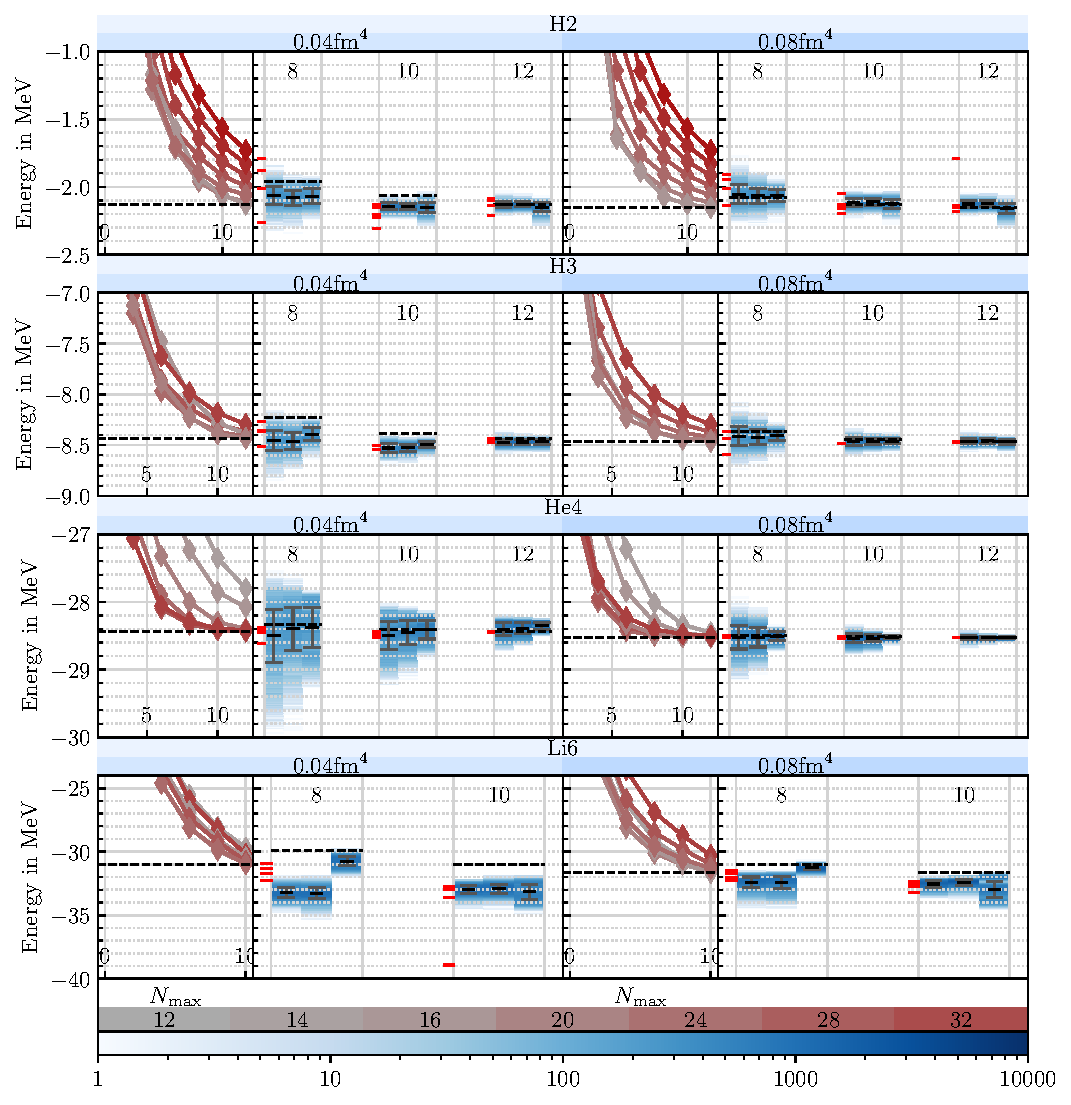
\includegraphics[width=\textwidth]{media/diff_evaluation.pdf}
  \caption{Evaluation of our training modes on the nuclei \n{2}{H}, \n{3}{H} and \n{4}{He} in the difference based extrapolation framework. The shown training modes are, in order from left to right, the basic training mode for comparison, the $N_\mathrm{max}$-limitation training mode and the SRG-filter training mode. For each nucleus and each flow parameter, the NCSM sequences are shown on the left (the different frequencies are colored respectively to the legend, which shows the frequencies $\hbar\Omega$ in \si[]{\mega\electronvolt}) and the extrapolations for a given maximum $N_\mathrm{max}$ on the right. For each maximum $N_\mathrm{max}$, the variational boundary is shown as a dashed line, and the classical extrapolations are shown as red ticks.}
  \label{fig:eval_diff}
\end{figure}


\section{conclusion}
In this chapter, we have introduced a second framework for extrapolating ground-state energies using neural networks. Here, we did not directly input the absolute energies into the network in return of an absolute energy prediction, but calculate the differences of consecutive energies in our sequences to input into the network. The output of the network was then trained on a prediction target calculated using the average distance of the last values in the formatted sequences to the actual limit. As a consequence, the evaluation process had to reconstruct the absolute energy prediction by adding the average energy for the highest $N_\mathrm{max}$ back onto the networks prediction of the difference.

In order to further examine the training modifications done in the previous chapter, we have evaluated our three training nuclei \n{2}{H}, \n{3}{H} and \n{4}{He} using the additional training modifications.

We have found that the difference-based extrapolation framework generally produced predictions with a smaller uncertainty. Further, the extrapolations generated were more reasonable than those generated by our previous absolute-based framework, as they were generally too low for small $N_\mathrm{max}$ values.

As for the training modes, we have found that they do not impact the absolute value of the prediction as much as in the absolute-based framework. Here, they have impacted the uncertainties of the predictions, where the SRG-filter training mode generally impacted the improvement of the uncertainties the most.
Before we reach a final decision on the two different frameworks and the three training modes, we will test how they affect the extrapolation of the nucleus \n{6}{Li} in the next chapter, which will be closer to a real use-case of extrapolation methods.

